\chapter{Diagramas y Topologías de Red}
\label{AppendixA}

En este apéndice se presentan versiones ampliadas de los diagramas incluidos en el Capítulo~\ref{chap:diseno_implementacion}. Su propósito es facilitar la lectura de etiquetas, relaciones de red y recorridos de tráfico que, por razones de escala, en el cuerpo principal del documento se muestran de forma resumida. Los diagramas fueron elaborados con la herramienta FossFLOW \cite{fossflow_github}.

\section{Topología General de la Infraestructura}
\label{AppendixA:TopologiaGeneral}

La Figura~\ref{fig:topologia_ampliada} reproduce en mayor tamaño la topología general de la infraestructura. Esta vista permite distinguir con más claridad las capas involucradas en el despliegue ---red externa, LAN institucional, contenedor LXC y servicios contenerizados--- y el recorrido del tráfico hasta la aplicación.

\begin{figure}[H]
    \centering
    \includegraphics[width=\textwidth,height=0.88\textheight,keepaspectratio]{figuras/capitulo3/TopologiadeRedyArquitecturaGeneral.png}
    \caption[Topología general de la infraestructura]{Vista ampliada de la topología general de la infraestructura y del flujo de tráfico entre WAN, LAN institucional y entorno contenerizado.}
    \label{fig:topologia_ampliada}
\end{figure}

\newpage

\section{Arquitectura Interna de la PaaS y Servicios Contenerizados}
\label{AppendixA:Coolify}

La Figura~\ref{fig:zoom_coolify_anexo} amplía la arquitectura interna de la PaaS Coolify. En ella se distinguen el contenedor LXC base, las redes virtuales de Docker y la separación entre la capa de control de la plataforma y los servicios desplegados sobre ella.

\begin{figure}[H]
    \centering
    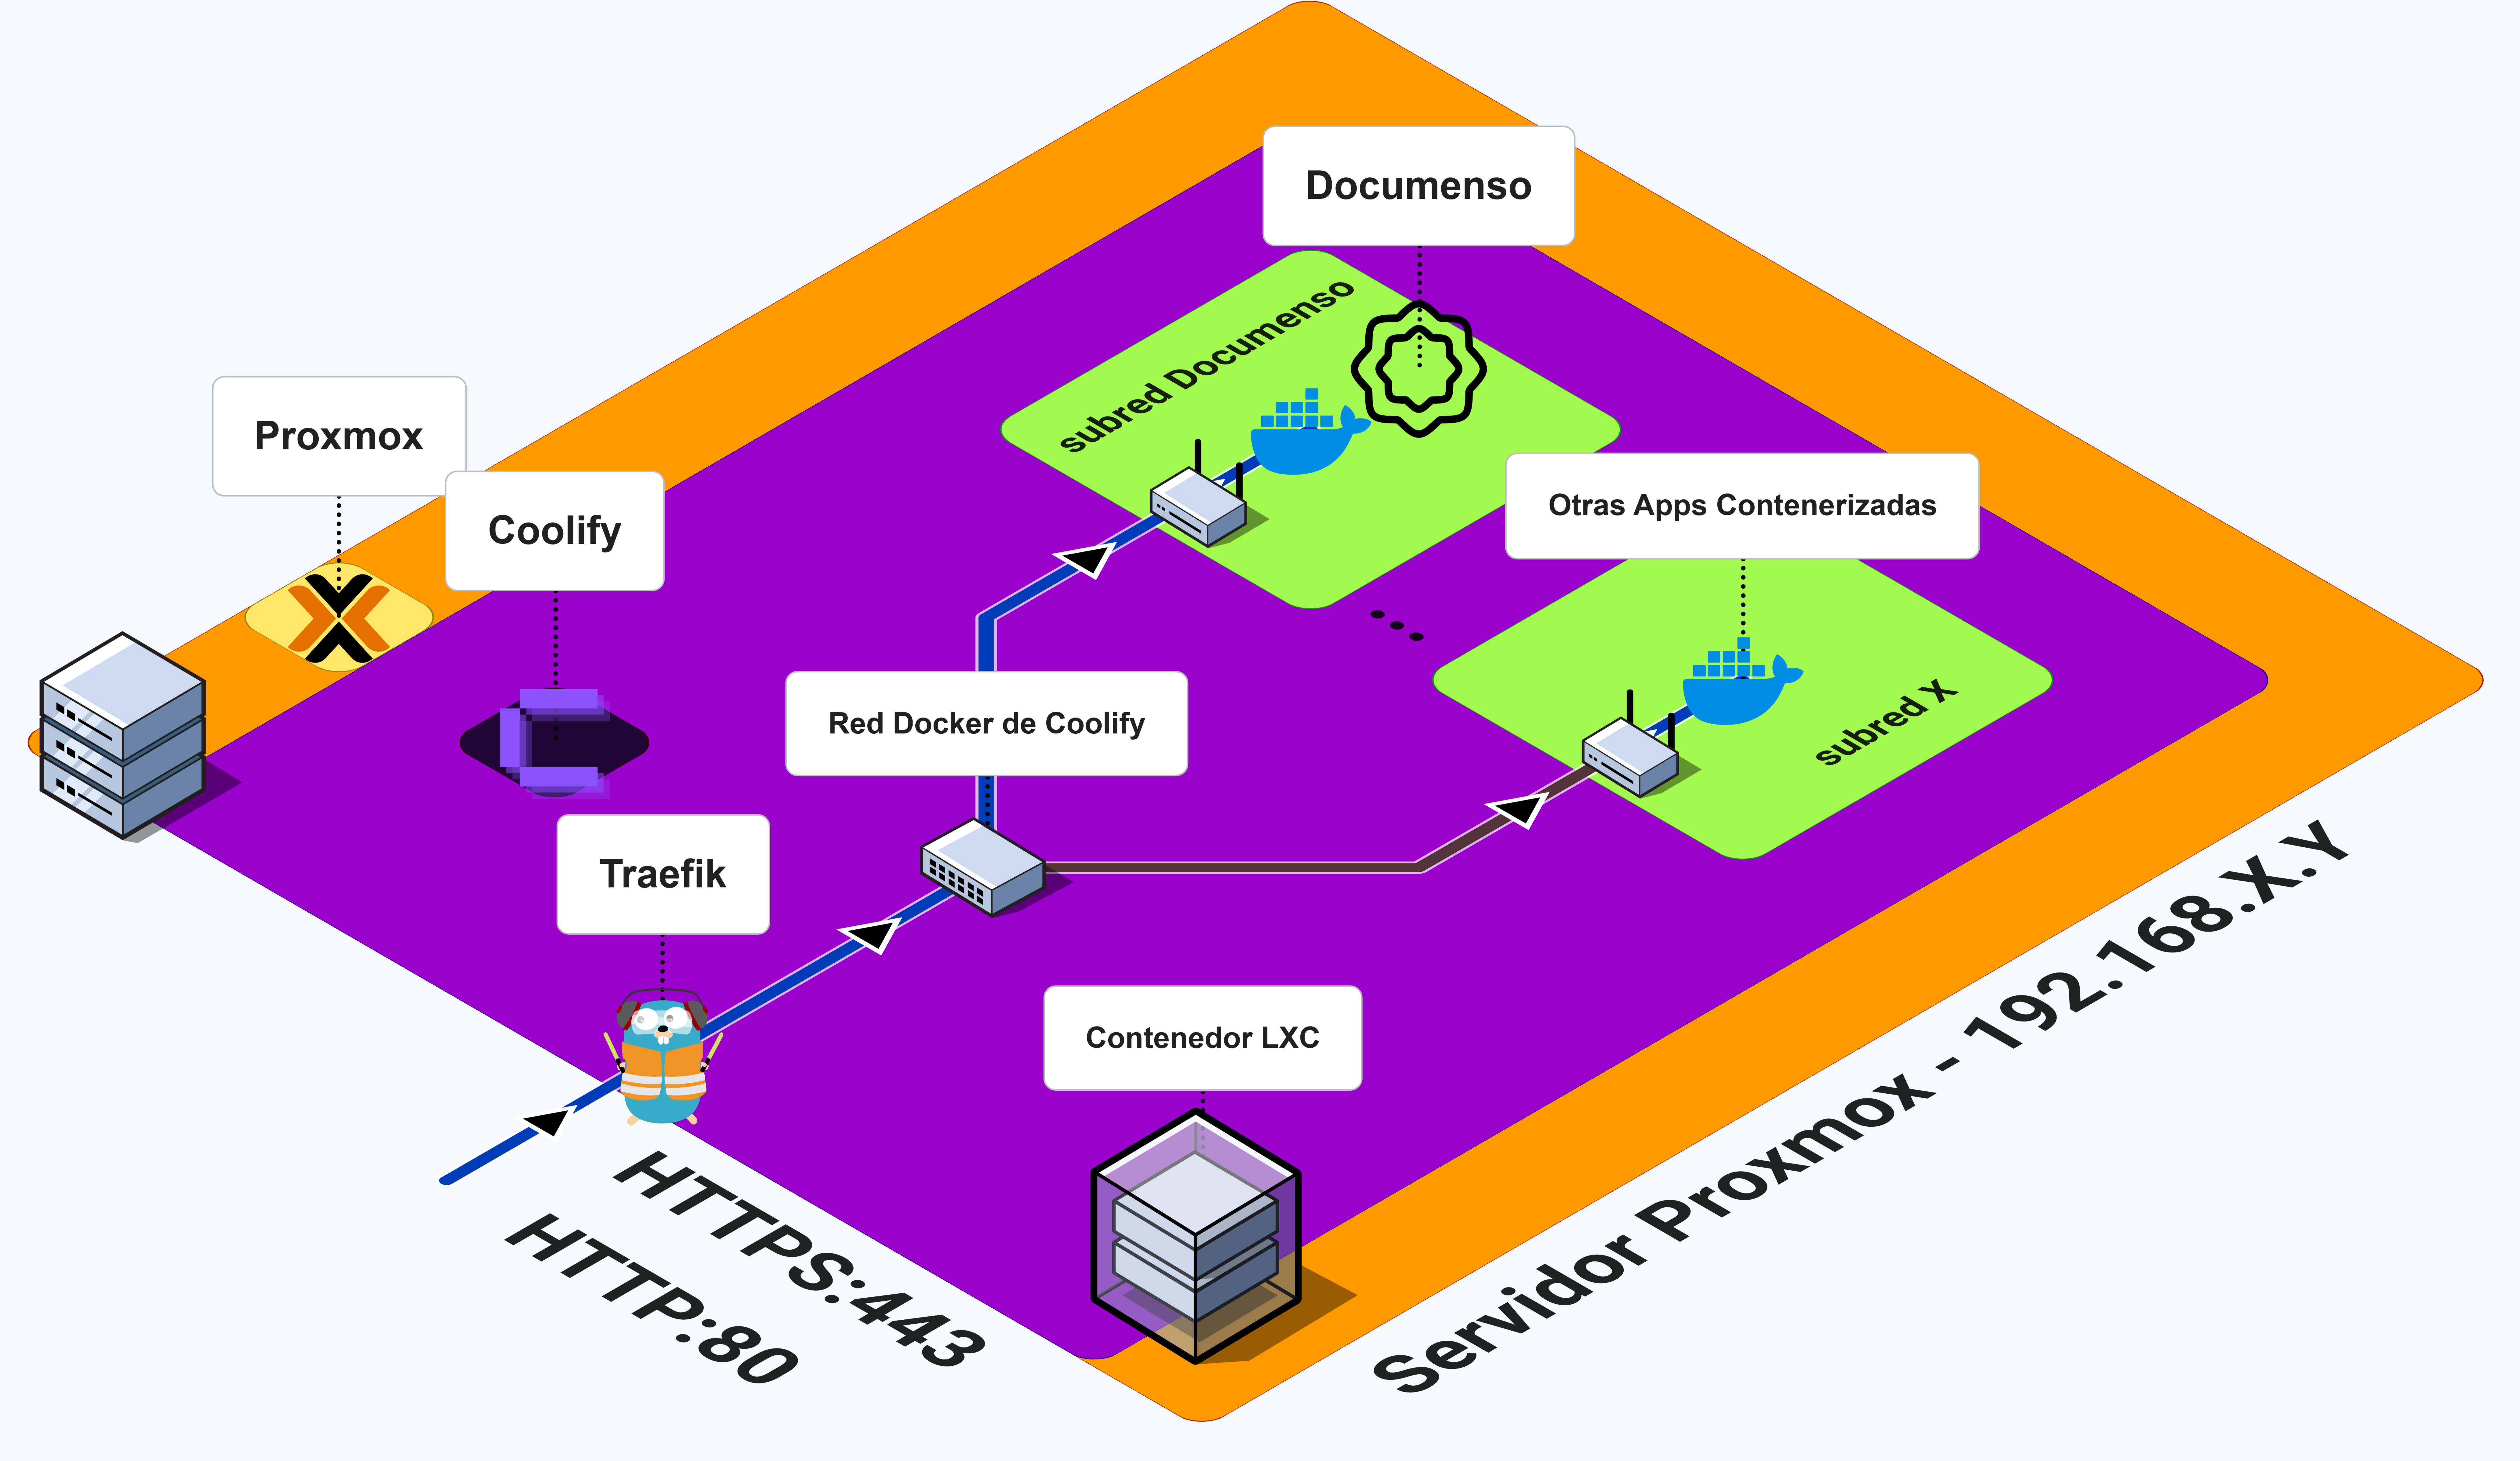
\includegraphics[width=\textwidth,height=0.88\textheight,keepaspectratio]{figuras/capitulo3/ZoomProxmoxCoolify.png}
    \caption[Arquitectura interna de la PaaS y servicios contenerizados]{Vista ampliada de la arquitectura interna de Coolify y de la segmentación de redes entre los servicios contenerizados desplegados en el LXC base.}
    \label{fig:zoom_coolify_anexo}
\end{figure}


\newpage

\section{Topología Interna de la Red Docker del Stack Documenso}
\label{AppendixA:RedDocker}

La Figura~\ref{fig:red_docker_anexo} amplía la topología interna del despliegue de Documenso. Esta vista permite identificar con mayor precisión los servicios del \textit{stack}, sus dependencias internas y el rol de Traefik como punto de entrada a la red privada administrada por Coolify.
\begin{figure}[H]
    \centering
    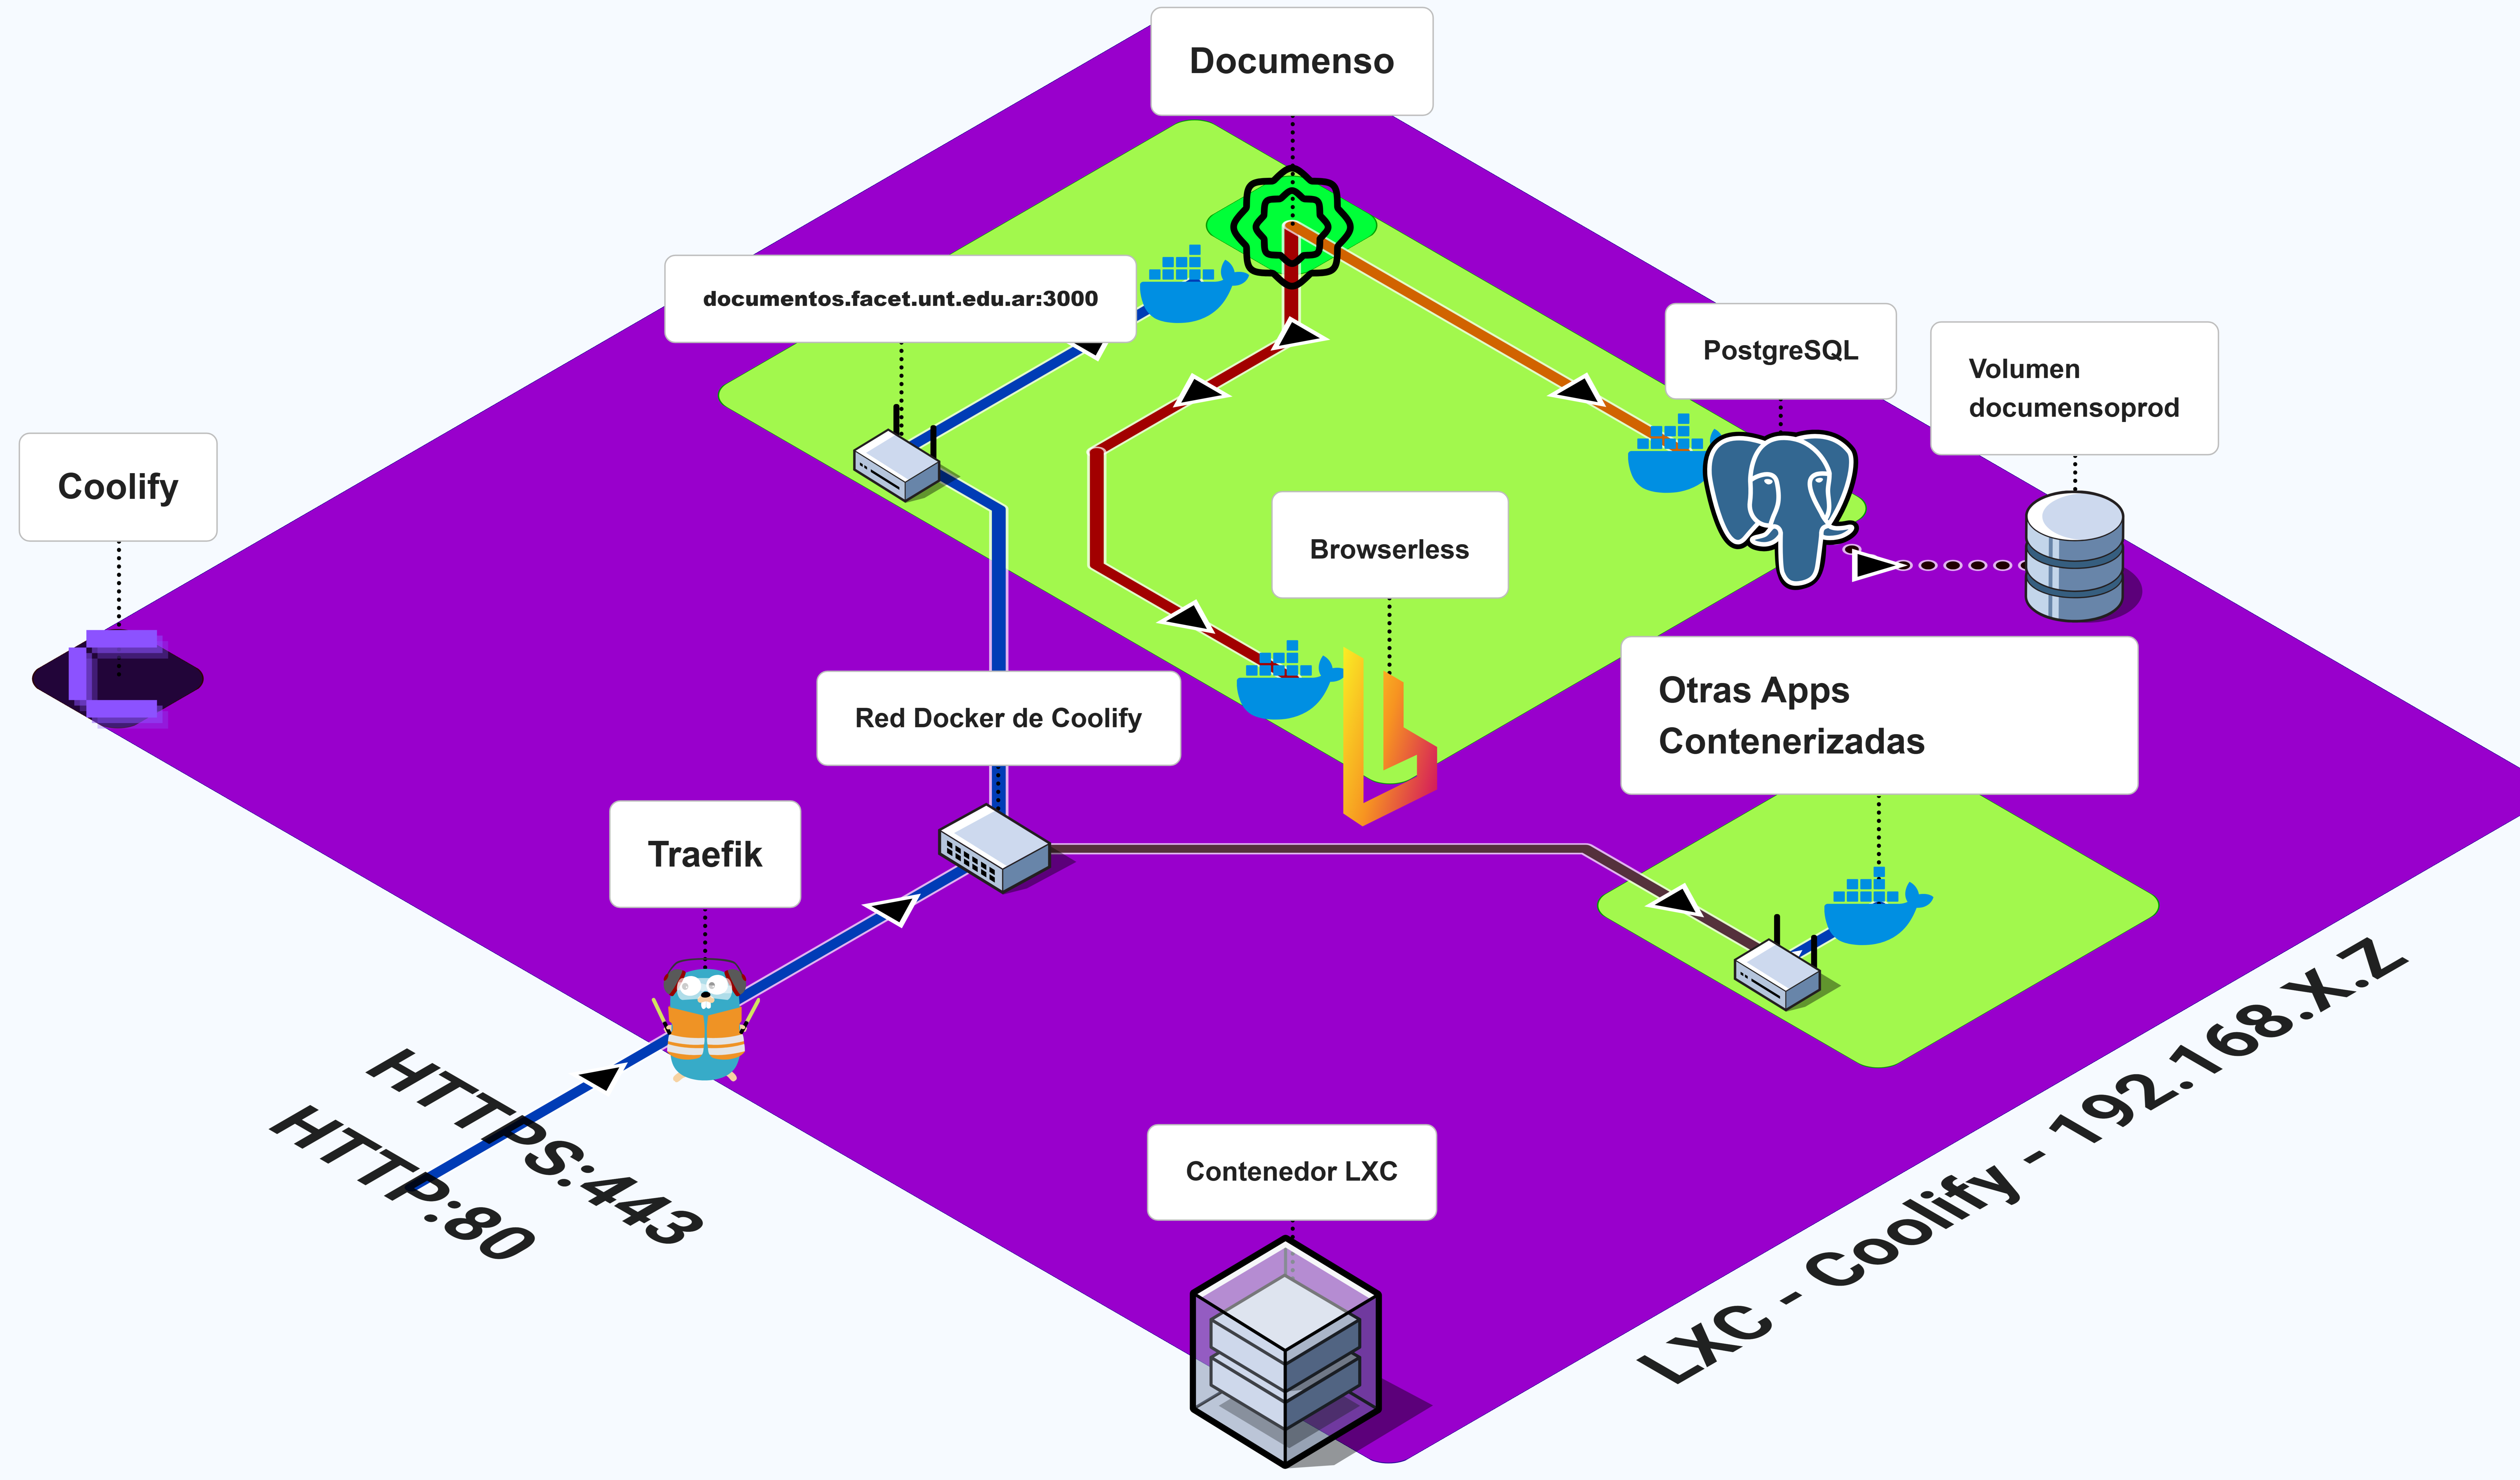
\includegraphics[width=\textwidth,height=0.88\textheight,keepaspectratio]{figuras/capitulo3/3.3.png}
    \caption[Topología interna de la red Docker del \textit{stack} Documenso]{Vista ampliada de la comunicación entre servicios contenerizados y del enrutamiento de Traefik dentro de la red privada del \textit{stack} desplegado por Coolify.}
    \label{fig:red_docker_anexo}
\end{figure}

\newpage

\section{Flujos de Acceso a MinIO a Través del Proxy Socat}
\label{AppendixA:FlujoMinIO}

La Figura~\ref{fig:flujo_minio_anexo} amplía el esquema de conectividad con MinIO descrito en la Sección~\ref{sec:proxy_socat}. Las líneas discontinuas representan los dos flujos que llegan al dominio público de almacenamiento: En verde el flujo directo originado en el navegador para recursos gráficos y en naranja el flujo indirecto originado en el \textit{backend} de Documenso para la gestión de documentos PDF. A partir de su convergencia en el reverse proxy perimetral, el recorrido común se muestra mediante líneas continuas a través de Traefik, el contenedor \texttt{socat} y el servidor físico TrueNAS/MinIO.

\begin{figure}[H]
    \centering
    \includegraphics[width=\textwidth,height=0.88\textheight,keepaspectratio]{figuras/capitulo3/3.4.png}
    \caption[Flujos de acceso a MinIO a través del proxy Socat]{Vista ampliada de la convergencia del flujo directo del navegador y del flujo indirecto del \textit{backend} hacia el servidor físico TrueNAS/MinIO, a través del reverse proxy perimetral, Traefik y el contenedor Socat.}
    \label{fig:flujo_minio_anexo}
\end{figure}
